
\documentclass[numbertotal,toc,wide]{../bpslides}

\usepackage{blindtext}

\definecolor{green0}{rgb}{0,0.5,0}
\definecolor{red0}{rgb}{0.8,0,0}
\definecolor{blue0}{rgb}{0,0.2,0.8}
\definecolor{black0}{rgb}{0,0,0}
\definecolor{orange0}{rgb}{1,0.25,0}
\definecolor{magenta0}{cmyk}{0,1,0,0}
\definecolor{purple0}{rgb}{0.5,0,1}

%%%%%%%%%%%%%%%%%%%%%%%%

\title{Title of your presentation}

\subtitle{Subtitle of the presentation}

\author{Author 1\inst{1} \and Author 2\inst{2} \and Author 3\inst{3}}

\institute{\inst{1} Institution 1, \  \inst{2} Institution 2, \  \inst{3} Institution 3}

\conference{Conference/university hosting the talk}

\date{\today}

\disclaimer{The opinions and analyses in this paper are the responsibility of the authors and, therefore, do not necessarily coincide with those of their employers.}

\foot{Whatever you want to write}

%%%%%%%%%%%%%%%%%%%%%%%%

\begin{document}

\begin{frame}[plain]
	\titlepage
\end{frame}

\begin{frame}{Main options}\label{firstslide}
	\begin{itemize}
		\item \texttt{numbering}: include slide numbers in the (right) footer
		\item \texttt{numbertotal}: include slide number and total number of slides in the (right) footer
		\item \texttt{toc}: include a table of contents at the beginning of each section and include the section title in the (right) footer.
		\begin{itemize}
			\item If this option is not selected but the user defines sections in the document, headings will show up in a separate slide at the beginning of each section and no section title will appear in the footer.
		\end{itemize}
		\item \texttt{wide}: change the aspect ratio of the slides from 4:3 (default) to 16:9
	\end{itemize}
\end{frame}

\begin{frame}{Colors and fonts}
	\hfill
	\begin{minipage}{0.3\textwidth}
		Colors:
		\begin{itemize}
			\item {\color{green0}\texttt{green}} \note{(default)}
			\item {\color{red0}\texttt{red}}
			\item {\color{blue0}\texttt{blue}}
			\item {\color{orange0}\texttt{orange}}
			\item {\color{black}\texttt{black}}
			\item {\color{magenta0}\texttt{magenta}}
			\item {\color{purple0}\texttt{purple}}
		\end{itemize}
	\end{minipage}
	\begin{minipage}{0.3\textwidth}
		Fonts:
		\begin{itemize}
			\item \texttt{sans} \note{(default)}
			\item \texttt{helvetica}
			\item \texttt{palatino}
			\item \texttt{bookman}
			\item \texttt{termes}
			\item \texttt{adventor}
			\item[]
		\end{itemize}
	\end{minipage}
	\hfill \ 
\end{frame}


\section{Itemize and enumerate environments}

\subsection{Itemize environment}

\begin{frame}{Itemize}\label{firstslide}
Lorem ipsum dolor sit amet, consectetur adipiscing elit, sed do eiusmod tempor incididunt ut labore et dolore magna aliqua. 
	\begin{itemize}
		\item Lorem ipsum dolor sit amet, consectetur adipiscing elit, sed do eiusmod tempor incididunt ut labore et dolore magna aliqua.
		\item Lorem ipsum dolor sit amet, consectetur adipiscing elit, sed do eiusmod tempor incididunt ut labore et dolore magna aliqua.
		\begin{itemize}
			\item Lorem ipsum dolor sit amet, consectetur adipiscing elit, sed do eiusmod tempor incididunt ut labore et dolore magna aliqua.
		\end{itemize}
		\item Lorem ipsum dolor sit amet, consectetur adipiscing elit, sed do eiusmod tempor incididunt ut labore et dolore magna aliqua.
	\end{itemize}
\end{frame}

\begin{frame}{Enumerate}{This is how a frame's subtitle looks like}
Lorem ipsum dolor sit amet, consectetur adipiscing elit, sed do eiusmod tempor incididunt ut labore et dolore magna aliqua. 
	\begin{enumerate}
		\item Lorem ipsum dolor sit amet, consectetur adipiscing elit, sed do eiusmod tempor incididunt ut labore et dolore magna aliqua.
		\item Lorem ipsum dolor sit amet, consectetur adipiscing elit, sed do eiusmod tempor incididunt ut labore et dolore magna aliqua. 
		\begin{enumerate}
			\item Lorem ipsum dolor sit amet, consectetur adipiscing elit, sed do eiusmod tempor incididunt ut labore et dolore magna aliqua. 
		\end{enumerate}
		\item Lorem ipsum dolor sit amet, consectetur adipiscing elit, sed do eiusmod tempor incididunt ut labore et dolore magna aliqua. 
	\end{enumerate}
\end{frame}

\section{Blocks and buttons}

\begin{frame}{Blocks}
	\begin{block}{Example of a block}
	Lorem ipsum dolor sit amet, consectetur adipiscing elit, sed do eiusmod tempor incididunt ut labore et dolore magna aliqua. Ut enim ad minim veniam, quis nostrud exercitation ullamco laboris nisi ut aliquip ex ea commodo consequat. Duis aute irure dolor in reprehenderit in voluptate velit esse cillum dolore eu fugiat nulla pariatur.
	\end{block}
	\begin{itemize}
		\item Lorem ipsum dolor sit amet, consectetur adipiscing elit, sed do eiusmod tempor incididunt ut labore et dolore magna aliqua.
		\item Lorem ipsum dolor sit amet, consectetur adipiscing elit, sed do eiusmod tempor incididunt ut labore et dolore magna aliqua.
	\end{itemize}
\end{frame}

\begin{frame}{Buttons}
	\vfill
	\begin{itemize}
		\item Lorem ipsum dolor sit amet, consectetur adipiscing elit, sed do eiusmod tempor incididunt ut labore et dolore magna aliqua.
		\item Lorem ipsum dolor sit amet, consectetur adipiscing elit, sed do eiusmod tempor incididunt ut labore et dolore magna aliqua.
		\item Lorem ipsum dolor sit amet, consectetur adipiscing elit, sed do eiusmod tempor incididunt ut labore et dolore magna aliqua.
		\item Lorem ipsum dolor sit amet, consectetur adipiscing elit, sed do eiusmod tempor incididunt ut labore et dolore magna aliqua.
	\end{itemize}
	\vfill
	\hfill An example of button $\to$ \button{firstslide}{back to first slide}
\end{frame}

\section{Tables and figures}

\begin{frame}{Tables}
	\begin{table}
		\centering
		\caption{Heading of the table}
		\begin{tabular}{cccc} \toprule
		& Mean & Median & Std Desvi.\\ \midrule
		Variable 1 & $1150$ & 900 & 235 \\ 
		Variable 2 & $430$ & 300 & 57 \\ 
		Variable 3 & $367$ & 210 & 113 \\ \bottomrule
		\end{tabular}
	\end{table}
\end{frame}

\begin{frame}{Figures}
	\begin{figure}
		\centering
		\caption{Heading of the figure}
		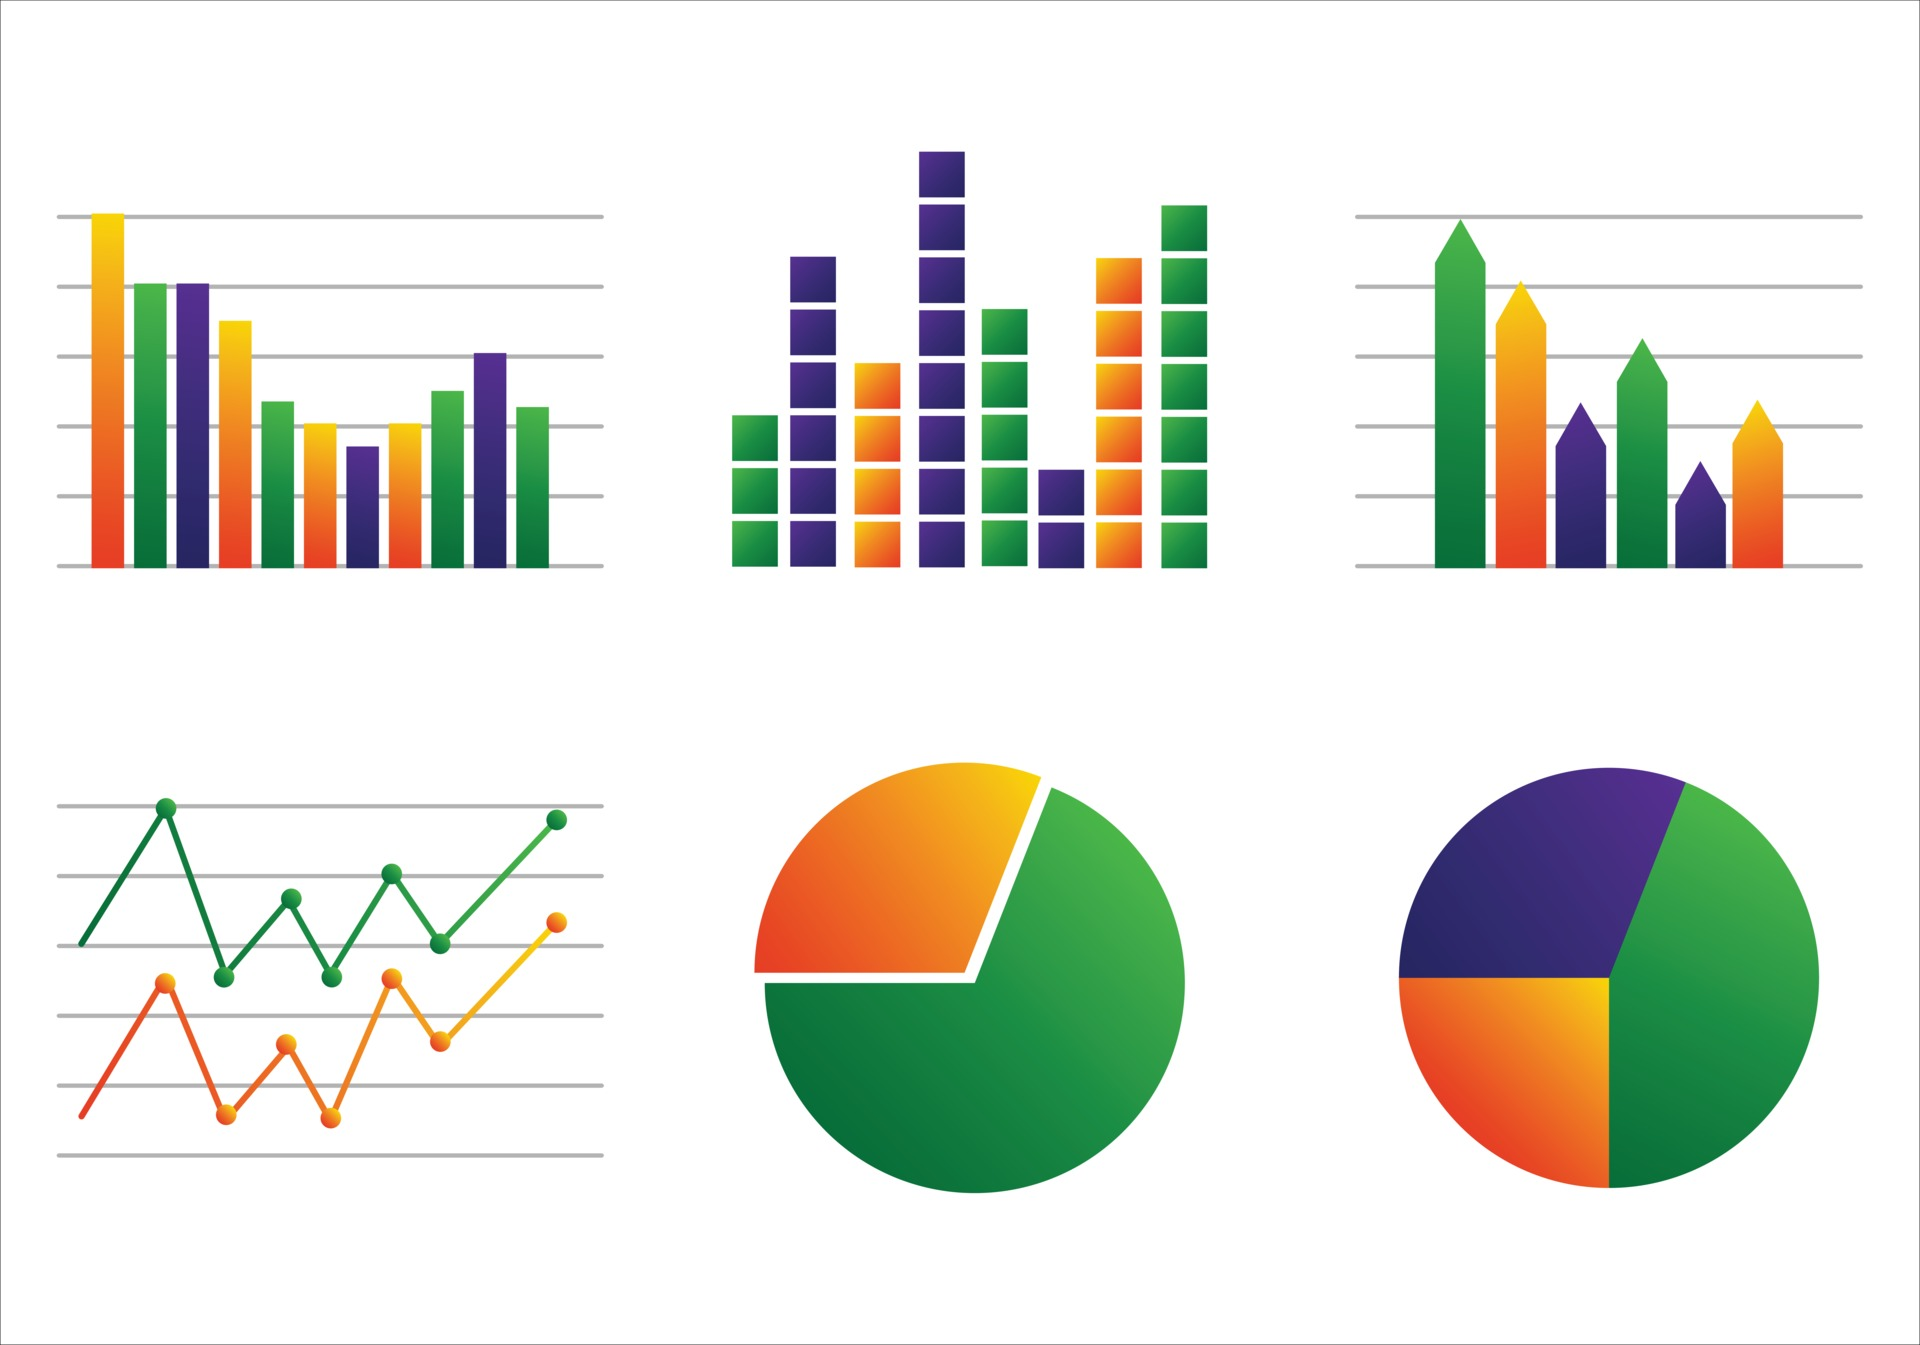
\includegraphics[width=0.9\paperheight]{graph}
	\end{figure}
\end{frame}

\section{New commands}

\begin{frame}{New commands - In preambule}
	\begin{itemize}
		\item \texttt{$\backslash$foot$\{$whatever$\}$} displays ``whatever'' in the bottom-left corner
		\item \texttt{$\backslash$conference$\{$the place$\}$} displays the place hosting the talk in the title page
		\item \texttt{$\backslash$disclaimer$\{$something$\}$} displays a footnote in the title page with a disclaimer
	\end{itemize}
\end{frame}

\begin{frame}{New commands - In main text}
	\begin{itemize}
		\item \texttt{$\backslash$paper$\{$Author$\}\{$Year$\}$} displays \paper{Author}{Year}
		\item \texttt{$\backslash$paperalt$\{$Author$\}\{$Year$\}$} displays \paperalt{Author}{Year}
		\item \texttt{$\backslash$alert$\{$Lorem ipsum$\}$} displays \alert{Lorem ipsum}
		\item \texttt{$\backslash$note$\{$Lorem ipsum$\}$} displays \note{Lorem ipsum}
		\item \texttt{$\backslash$under$\{$Lorem ipsum$\}$} displays \under{Lorem ipsum}
		\item \texttt{$\backslash$vs}: equivalent to \texttt{$\backslash$vspace$\{$0.1cm$\}$}
		\item \texttt{$\backslash$hs}: equivalent to \texttt{$\backslash$hspace$\{$0.1cm$\}$}
		\item \texttt{$\backslash$boxed$\{$Lorem ipsum$\}$} displays\\ \boxed{Lorem ipsum}
	\end{itemize}
\end{frame}

\begin{frame}{New commands - In math mode}
	\begin{itemize}
		\item \texttt{$\backslash$mathpause}: similar to \texttt{$\backslash$pause} but specifically design for display mode equations (the standard command typically adds a vertical space).
		\item \texttt{$\backslash$so}: displays $\so$
		\item \texttt{$\backslash$eqboxed$\{$x = 0$\}$} displays $x=0$ in a box.
		\begin{itemize}
			\item Example: \texttt{\$\$ x = exp(1) $\backslash$so $\backslash$eqboxed$\{$x = 0$\}$ \$\$ } displays
			$$x = \exp(1) \so \eqboxed{x=0}$$
		\end{itemize}
		\item \texttt{$\backslash$llave$\{$x = 0$\}$$\{$Lorem ipsum$\}$} displays $$\llave{x=0}{Lorem ipsum}$$
	\end{itemize}
\end{frame}

\begin{frame}[plain]{}
	\begin{center}{\Large
		\alert{Comments and suggestions are very welcome}\vs\vs\vs\vs\vs\vs\par \href{mailto:bpetit@cunef.edu}{bpetit [at] cunef.edu}
		}
	\end{center}
\end{frame}

\end{document}
